\chapter
 [Preliminaries]
 {Preliminaries}
\label{chp:background}


\begin{abstract}
    In this chapter we discuss some of the concepts that are relevant for understanding the rest of the thesis.
    We explain what we mean by quantum networks, what they can do, and how quantum network applications look like.
\end{abstract}

\section{Quantum networks}

A quantum network consists of devices that are connected together and that can establish entanglement between separate devices in that network.
More specifically, we assume quantum network to consist of \textit{nodes} that are connected by \textit{classical channels} and \textit{quantum channels}.
Classical channels enable classical communication between nodes, while quantum channels are used for \textit{entanglement} generation (\cref{background:sec:entanglement}) between nodes.
Within a quantum network, one can distinguish between two main types of nodes: First, there are \emph{end nodes}~\cite{wehner_2018_stages}, with which users execute quantum network applications (\cref{background:sec:applications}).
In classical networks, end nodes are laptops, phones or other devices.
In the quantum domain, end nodes may be simple photonic devices that can only create or measure quantum states, or they may be quantum processors capable of arbitrary qubit operations and storage of information within a quantum memory.
The type of end node dictates what applications are possible~\cite{wehner_2018_stages}, and we have chosen to focus on the most general form of an end node, namely, a quantum processor including quantum memory.
So, our goal is to enable programming and execution of arbitrary quantum network applications on end nodes that are quantum processors.
For the remainder of this thesis, we will thus always take end nodes to be quantum-processor end nodes.

Second, a quantum network can include \emph{intermediate nodes} that perform routines necessary to connect two or more end nodes (\cref{background:fig:network_model}).
We refer the reader with a background in computer science to~\cite{vanMeter_book} for a gentle introduction to quantum networks. 
Intermediate nodes, such as quantum-repeater nodes, are used to establish long-distance entanglement between remote end nodes.
These intermediate nodes may employ protocols such as entanglement swapping and entanglement distillation in order to realize end-to-end links with sufficiently high fidelity (quality) for network applications.
These protocols are handled by a network stack (see, e.g.~\cite{dahlberg_2019_egp}) that exists at each node.
The network stack includes a link layer, a network layer, a control plane, and other networking functions; it is responsible for entanglement generation.

Intermediate nodes do not execute user applications (i.e. the applications we focus on in this thesis), which is done only by end nodes. 
Therefore, only end nodes need to have an additional stack implementing the application layer in a network, which is referred to as an \emph{application stack} (see \cref{background:fig:network_model}).
The application stack is responsible for the execution of arbitrary user applications, and integrates with the network stack for entanglement generation over the network.
We remark that it is the purpose of a network layer~\cite{dahlberg_2019_egp, kozlowski_2020_qnp} to provide a service to the application layer that allows entanglement generation with remote end nodes.
Importantly, this service should not require the application layer to have any knowledge about the connectivity of the network.

\begin{figure}[t]
    \centering
    % 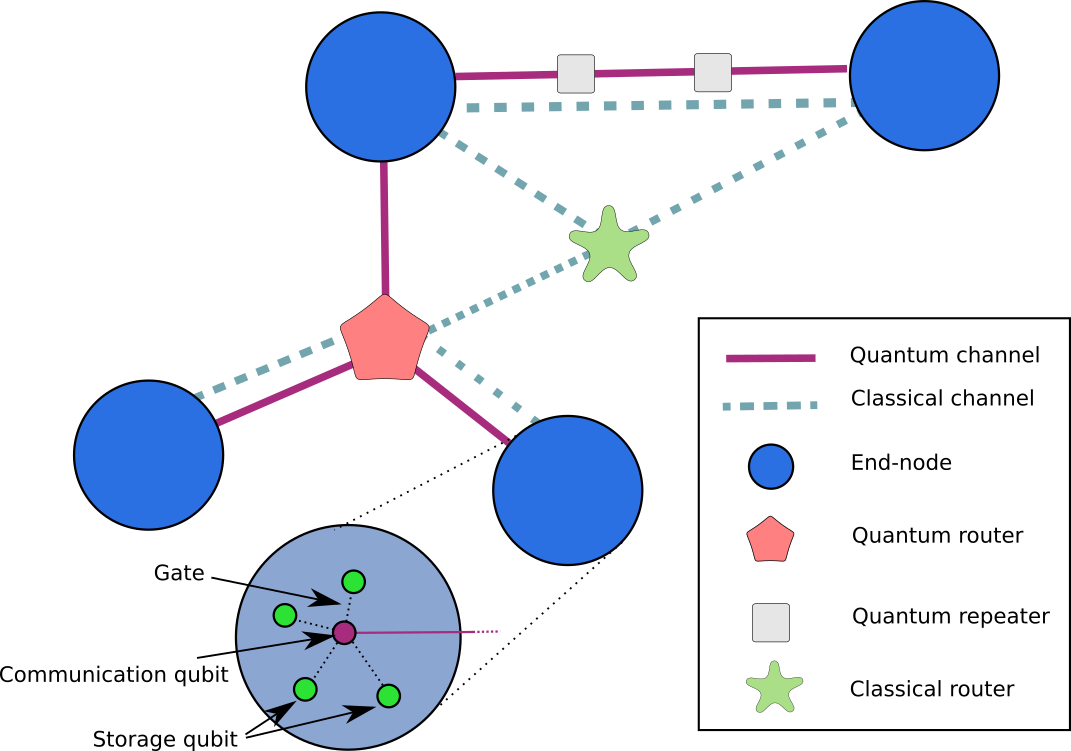
\includegraphics[width=0.4\linewidth]{figures/netqasm/network_model.png}
    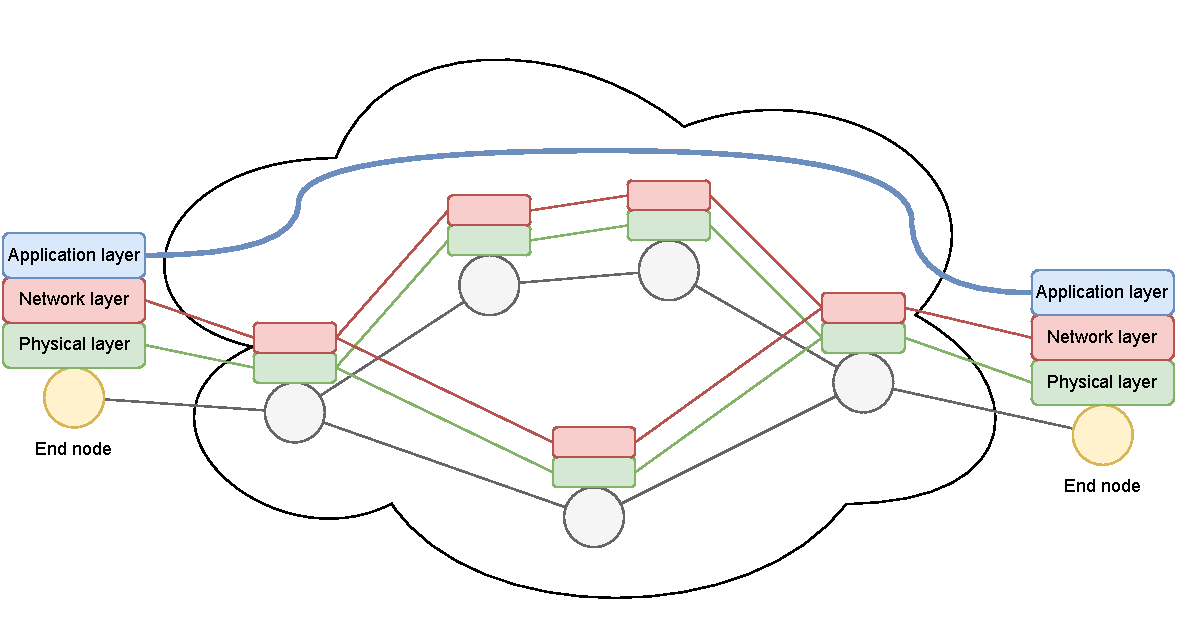
\includegraphics[width=0.8\linewidth]{figures/background/network_nodes.pdf}
    \caption{
        \textbf{Schematic overview of a quantum network.}
        A quantum network consists of nodes (yellow and grey circles) that are connected by classical and quantum communication channels (grey lines).
        Each node implements a physical layer (green boxes and lines) that enables entanglement generation with neighboring nodes.
        Each node also implements a network stack, including a network layer (red boxes and lines, which may be subdivided into a separate link layer and a network layer~\cite{dahlberg_2019_egp, kozlowski_2019_towards}).
        This layer realizes long-distance entanglement creation between nodes and may include protocols such as entanglement swapping and distillation.
        \newline
        We emphasize however that the focus of this work is to program and execute applications on the end nodes, i.e. enabling the application layer in networking terms.
        Only \emph{end nodes} (yellow circles) implement an additional application layer (blue boxes and line), which executes arbitrary user applications.
        From the perspective of this layer, end nodes are logically directly connected (blue line), and this layer is hence independent from implementations and protocols in the network layer and is only dependent on the service  provided by the network layer.
        Logically directly connected means that the application layer relies on the service of the network layer to enable end-to-end entanglement generation between end nodes and does not concern itself with how the entanglement is generated.
        This abstraction is a key element enabled by a quantum network stack such as~\cite{dahlberg_2019_egp} and exactly analogous to abstractions used in classical networking, where e.g. a web browser can be executed on a laptop independently of how the internet connection between the laptop and a web server is realized.
    }
    \label{background:fig:network_model}
\end{figure}

\subsection{End nodes}
\label{background:sec:end_nodes}

As mentioned above, end nodes in a quantum network possess a quantum processor acting on quantum memory.
Quantum memory consists of individual quantum bits (\emph{qubits}), each of which can have a quantum state, such as $\ket{0}, \ket{1}$ or $\ket{+}$ (see~\cite{nielsen_chuang_2002} for a an extensive introduction to qubits and quantum states).
The quantum network can deliver entangled pairs to end nodes, such that end nodes can obtain qubits in their quantum memory that are entangled with qubits in the quantum memory of other end nodes.
An end node also possesses a classical processor and a classical memory.
Furthermore, an end node can send and receive classical messages to and from other end nodes in the network.
These abilities (classical and quantum processing, as well as classical and quantum communication, the latter being entanglement generation) are all required for the execution of quantum network applications (\cref{background:sec:applications}).


% Quantum \textit{network} processors have additional challenges:
%     (1) the processor may have to act as a local computation unit and a network interface at the same time;
%     for example, in NV centers, an electron spin qubit is used for generating entanglement with a remote node but is also needed to do local two-qubit gates,
%     (2) remote-entanglement operations may not have a fixed time in which they complete, which makes scheduling and optimization more difficult.

\paragraph{Quantum memory}
Each quantum memory has a certain \textit{topology} that describes which operations can be applied on which (pair of) qubits.
Some of the qubits in a quantum memory may be used to create an entangled state with another node.
These qubits are called \emph{communication qubits}~\cite{dahlberg2019linklayer}, in contrast to \emph{storage qubits} which can only directly interact with other qubits part of the same local node.
A storage qubit may however hold a state that is entangled with a qubit in another node: after remote entanglement generation using a communication qubit, the state in that local qubit could be transferred to one of the storage qubits, preserving the remote entanglement.
Some hardware implementations only have a single communication qubit and multiple storage qubits~\cite{Bernien2014}, whereas others can have multiple communication qubits~\cite{Inlek2017}.

There are various quantum hardware implementations for quantum network processors, such as nitrogen-vacancy centers in diamond~\cite{pompili2021realization}, trapped ions~\cite{krutyanskiy2023entanglement}, and neutral atoms~\cite{hofmann2012heralded,ritter2012elementary}, which all have different capabilities and gates that can be performed.

\paragraph{Noise and decoherence}
All current quantum processor implementations are in the so-called \acf{NISQ} stage, meaning that they have a limited number of qubits (typically in the order of tens or a few hundred for (non-network) quantum computers, and only a handful of qubits for quantum network processors), and these qubits are susceptible to \emph{noise} and errors due to their limited \emph{coherence} (lifetime) and imperfect control.
Limited lifetime means that the quality of qubits decreases (called \emph{decoherence}) over time, eventually rendering them unreliable (computations produce random or incorrect results).
\todo{give concrete numbers of coherence times}
Decoherence may also happen by applying gates.
Gates transform the state of qubits, but typically also induce some noise, leading to decoherence of the qubit.

Therefore, the timing and duration of operations (such as local gates or entanglement generation with another node) have an impact on the quality of quantum memory, and indirectly on the performance of applications.

Throughout this thesis, when we say `qubit', these may be physical qubits, but may also be logical qubits (multiple physical qubits together representing one more robust usable qubit) in case the end node does error correction~\cite{lidar2013quantum}.




% \paragraph{Hybrid classical-quantum processing}
% Hybrid classical-quantum programs are used to realize e.g. \textit{variational quantum eigensolvers (VQE)}~\cite{diadamo2021distributed, liu2022layer} or \textit{quantum approximate optimization algorithms (QAOA)}~\cite{farhi2014quantum}.
% For such programs, a quantum circuit is executed, followed by some classical processing, and a next circuit is issued.


\subsection{Entanglement generation}
\label{background:sec:entanglement}
Entanglement is a phenomenon in quantum physics where two or more particles (qubits) are correlated in a way that is not possible classically. In a quantum network, such entangled qubits may be established across separate nodes, realizing a quantum connection between those nodes. Entanglement can be used by quantum network applications as a resource in order to realize applications~\cite{wehner_2018_stages} that are impossible with classical networks, including applications such as data consistency in the cloud~\cite{benor_2005_byzantine}, privacy-enhancing proofs of deletion~\cite{poremba_quantum_2022}, exponential savings in communication~\cite{guerin_exponential_2016}, or secure quantum computing in the cloud~\cite{broadbent_2009_ubqc,childs_2005_secure_qc}.

In order for two neighboring quantum network nodes to produce entanglement between them, they need to simultaneously perform an action to trigger entanglement generation (at the physical layer, synchronized to nanosecond precision).
This means neighboring quantum network nodes need to perform a network operation (entanglement generation) in a \emph{very specific} time slot in which they make an attempt to generate entanglement.
Such time slots are generally aggregated into larger time bins, corresponding to making batches of attempts in time slots synchronized at the physical layer.
We refer to e.g.~\cite{pompili_2022_experimental} for background information on the physical layer of entanglement generation in quantum networks, and the readers with a background in computer science to e.g.~\cite{dahlberg_2019_egp} for a detailed explanation of scheduling of entanglement generation in quantum networks.

In short, network operations in quantum networks need to be executed by the node at very specific time bins.
These time bins cannot be determined by the quantum node itself.
Instead selection of time bins for a specific quantum operation require agreement with the neighboring node~\cite{dahlberg_2019_egp} (and more generally with the quantum network when the end-to-end entanglement is made via intermediate network nodes, \cref{background:fig:network_model}) by means of a network schedule, e.g. determined by a (logically) centralized controller, see Ref.~\cite{skrzypczyk_2021_arch}.

\paragraph{Quantum network stack}
A quantum network stack has been proposed~\cite{dahlberg2019link} and implemented~\cite{pompili2022experimental} that turns entanglement generation into a robust service independent of the quantum hardware platform.
Important for the design of an architecture for the execution of quantum network applications is that in this stack, the nodes will establish a network schedule of time slots in which they will trigger entanglement generation (due to need to synchronize entanglement generation as mentioned above).
This means that once entanglement has been requested from the network, the nodes can use only the slots in the network schedule to produce entanglement between them, imposing constraints on the ability to schedule applications. What's more, in present day systems~\cite{pompili2021realization, krutyanskiy2023entanglement} limitations in the physical devices prohibit the execution of local operations while engaging in network operations (entanglement generation), creating further dependencies between the local quantum execution and entanglement generation. 
As the specifics of network scheduling~\cite{network-scheduling, skrzypczyk2021architecture} are not within scope of this thesis, we assume the existence of a \textit{network controller} that takes application demand for entanglement and issues a network schedule to the nodes. 
A schedule consists of sequential time slots, each with a start time and duration, when the node will trigger entanglement generation.
Nodes are not forced to attempt entanglement in corresponding time slots, and can instead choose to do local processing instead.




\section{Programs and applications}
\label{background:sec:applications}

In this section we discuss what (quantum network) applications and programs are, and how they are represented.

\subsection{Quantum computing}
First, let us briefly discuss quantum \emph{computing} (rather than networking).
A quantum computing program runs on a single quantum processor, which may be an individual node in a quantum network, but may also just be a standalone quantum computer.
A quantum computing program consists of performing operations on qubits.
A quantum program for local (non-network) quantum computing is typically represented as a \emph{quantum circuit}.
A circuit describes the program's quantum memory --- as individual qubits --- and the gates that are applied on these qubits.
When visualized, like in \cref{background:fig:local_circuit}, qubits are represented by horizontal lines and operations by boxes on those lines.
Such circuits must be read from left to right: gates on the left are applied first, then the ones to the right and so on.

\begin{figure}[t]
    \centering
    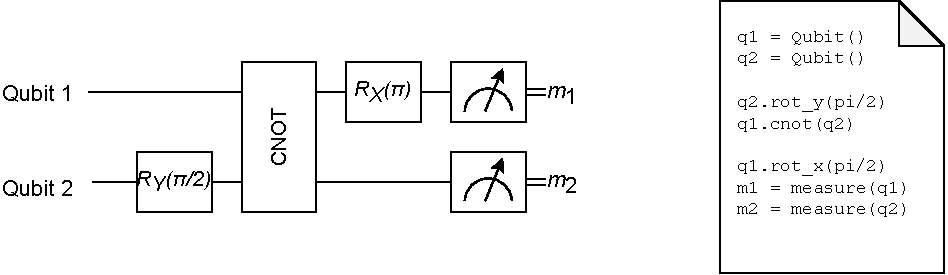
\includegraphics[width=0.8\linewidth]{figures/background/local_circuit.pdf}
    \caption{
        Two representations of an example quantum program using two qubits.
        This program can run on a quantum computer, which may be a node in a quantum network.
        Left: circuit model of the program.
        A horizontal line represents a single qubit.
        Blocks are quantum gates applied on qubits; there are single-qubit gates (such as a rotation gate around axis $X$ with angle $\pi$ ($R_X(\pi)$) and multi-qubit gates (such as a CNOT; note that a CNOT gate is also sometimes depicted as a vertical line and an XOR symbol on one of the qubits).
        Time goes from left to right, so the gates are applied in the order (left to right) they are depicted.
        A measurement `gate' destroys the qubit and produces a classical bit, depicted by a double line.
        Right: the same program but represented in a programming language (language shown is fictional and for illustration purposes only; in \cref{chp:netqasm} we present a real, detailed language).
        This is what a developer might write when programming (`coding') the program.
    }
    \label{background:fig:local_circuit}
\end{figure}

Operations include quantum \emph{gates} (such as rotation gates or the Hadamard gate), initialization, and measurement (readout).
Quantum gates may be on a single qubit, or on multiple qubits.
For example, the CNOT gate used in the example of \cref{background:fig:local_circuit} is a 2-qubit gate.
The code, or the `recipe' of quantum programs is hence classical, while the information and memory that the program manipulates is quantum.
Besides quantum operations, there may be limited classical control, such as a gate being executed depending on a measurement outcome.
Typically, a quantum circuit is executed in one go, on a very small timescale.
Quantum memory used for quantum computing~\cite{de_leon_materials_2021} often only stays coherent (alive and useful) for microseconds.
For more information on quantum computing, see e.g.~\cite{nielsen_chuang_2002}.

Quantum computing does not necessarily involve only quantum circuit execution with limited classical control.
\emph{Hybrid classical-quantum} programs consist of an interleaving of purely classical computation and quantum circuit execution.
For example, in \acf{VQE}~\cite{diadamo2021distributed, liu2022layer} and \acf{QAOA}~\cite{farhi2014quantum},
upon completion of a quantum circuit, the classical results are processed, resulting in a new quantum circuit that is then executed; this process repeats multiple times.

\subsection{Quantum network applications}
Quantum network applications, also called \textit{protocols}, are multi-partite programs that involve entanglement generation and classical communication between different end nodes, as well as local computation.
The local computation includes arbitrary classical computation as well as local quantum operations (like in quantum computing circuits, see above).
Examples include Quantum Key Distribution (QKD)~\cite{bb84, ekert_1991_e91}, leader election protocols~\cite{kobayashi2014simpler, ganz2009quantum}, and Blind Quantum Computation (BQC)~\cite{Wehner2018stages}.
In this thesis, we consider quantum network applications in the quantum memory stage~\cite{wehner_2018_stages} and above. That is, applications that require the use of a quantum processor that can manipulate and store qubits. For simpler applications in the prepare-and-measure and entanglement generation stages~\cite{wehner_2018_stages}, e.g. quantum key distribution~\cite{bb84Original,ekert_1991_e91}, where the quantum states are immediately measured by the nodes, it would be sufficient to realize a system implementing a quantum network stack and classical processing only.

\begin{figure}[t]
    \centering
    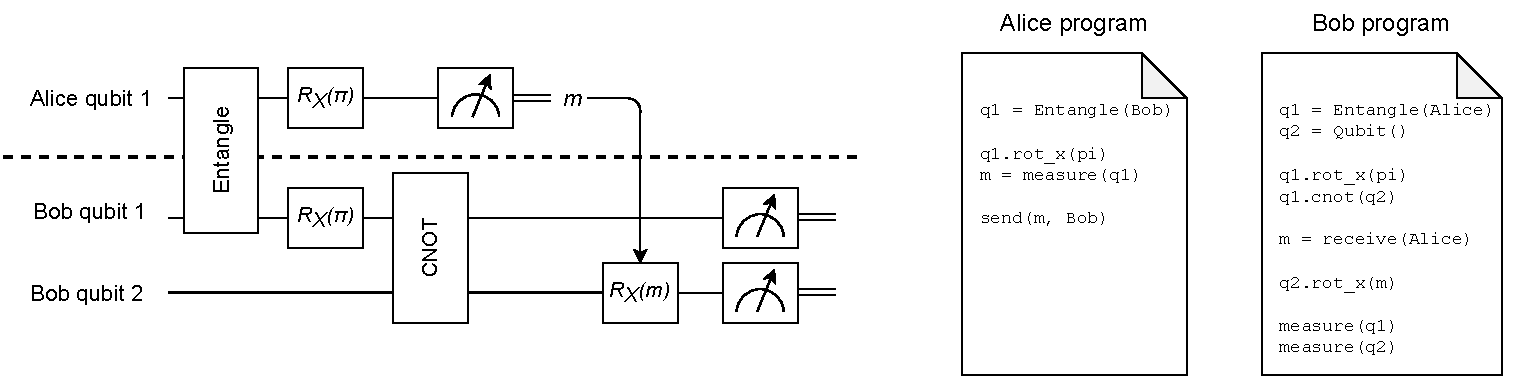
\includegraphics[width=1.0\linewidth]{figures/background/2node_circuit.pdf}
    \caption{
        Two representations of an example two-node quantum network application.
        The application is run on the nodes Alice (possessing one qubit) and Bob (possessing two qubits).
        Left: circuit model of the application.
        The Entangle operation is depicted here as a two-qubit gate; however since it acts on qubits in different nodes (Alice and Bob),
        this is not as trivial as a local two-qubit gate such as the CNOT, and instead requires coordination between the two nodes.
        Furthermore, classical communication may happen in the form of sending a message.
        In this case, after measuring her qubit, Alice sends the classical outcome bit $m$ to Bob.
        Bob then uses this in his local X-rotation gate.
        Right: the same application but represented as two separate programs written in a programming language.
        Since Alice and Bob are separated nodes, they each program their own local code.
        This code may however include external operations, such as entanglement creation with the other node, and sending or receiving messages.
        Note that these operations must match --- something they are responsible for themselves, by e.g. following some pre-established protocol.
    }
    \label{background:fig:2node_circuit}
\end{figure}


\subsection{Programs}
Throughout this thesis, we will use the following terminology.
\emph{Applications} refer to multi-node protocols or use-cases of quantum networks, such as QKD and BQC.
\emph{Programs} refer to the code that is run on individual quantum network nodes.
Applications are realized by the joint execution of programs on their respective nodes.

A multi-node quantum network application is hence partitioned into separate single-node programs that run concurrently on different network end nodes (e.g. in BQC: a client program on a client node and a server program on a server node, or in secret sharing~\cite{hillery1999quantum}: a program each on many nodes).
Each of these programs runs independently, and may also be independently programmed (and compiled).
This highlights the difference with distributed quantum computing (see e.g.~\cite{cacciapuoti2019quantum}), where all nodes can be accessed and controlled by a single program. 



\paragraph{Program ingredients}

\begin{figure}% [ht]
    \centering
    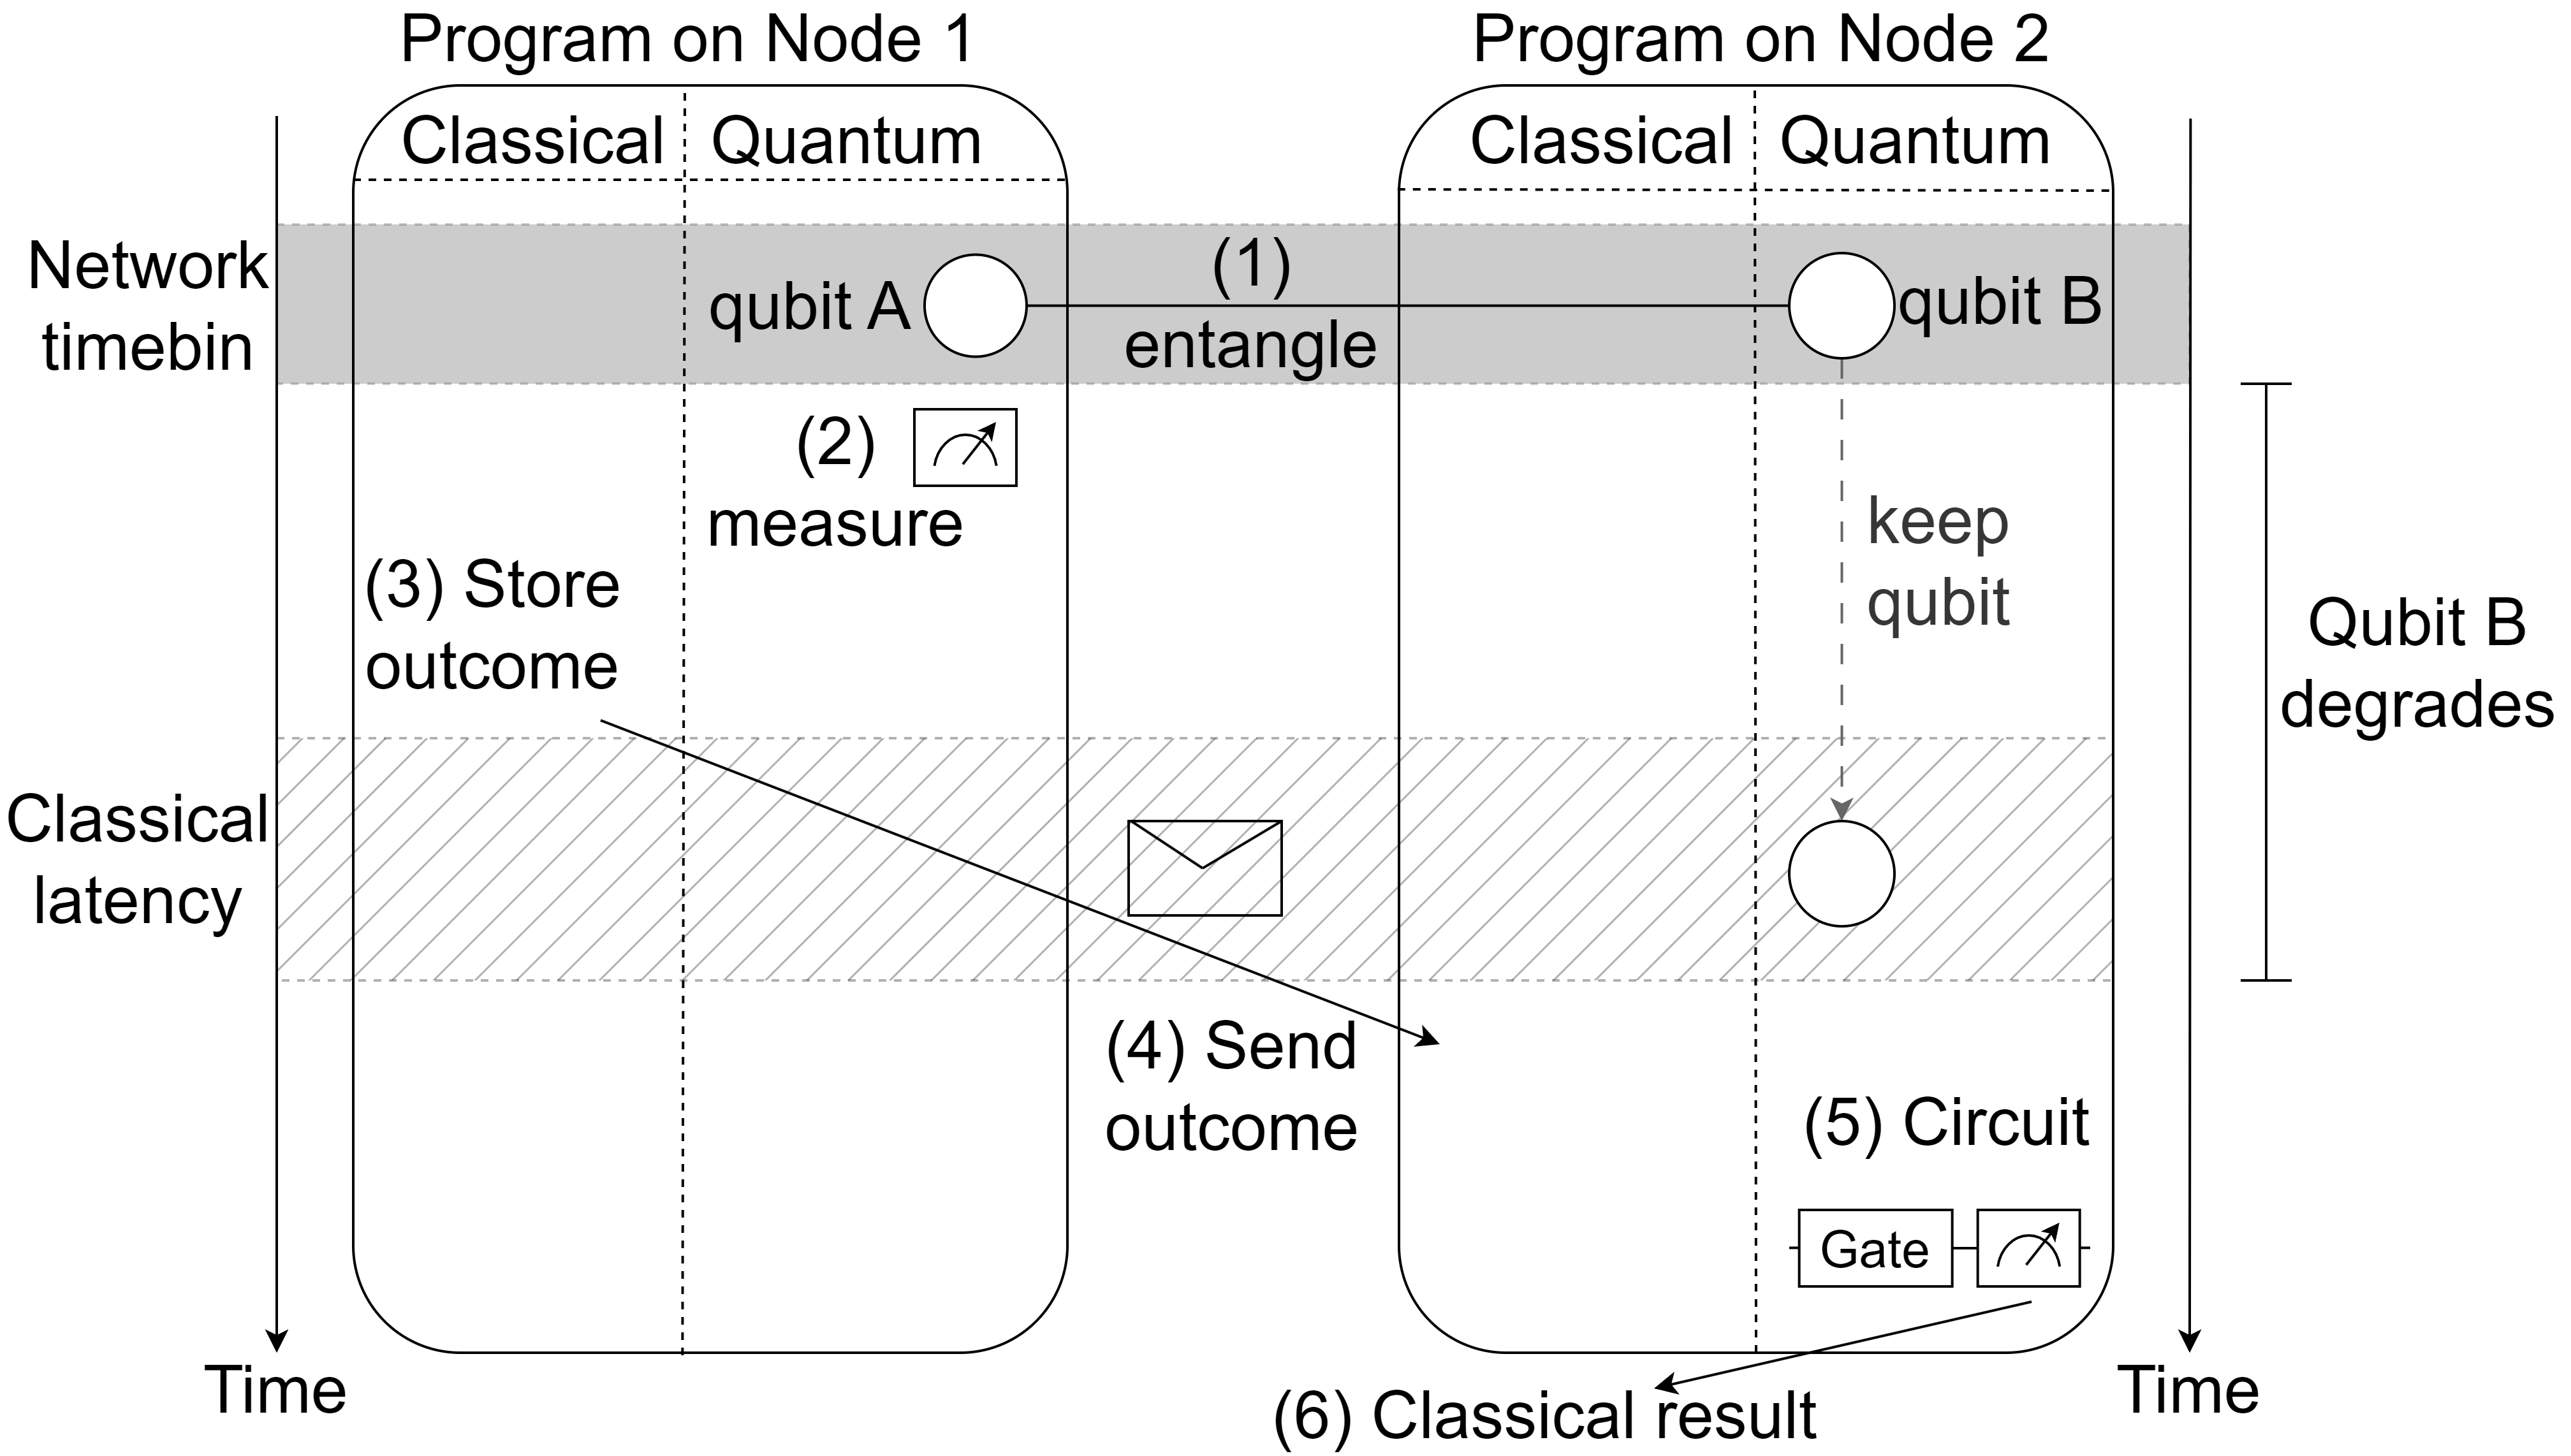
\includegraphics[scale=0.35]{figures/qoala/program_illustration.png}
    \caption{Another visualization of a quantum network application, focusing on the different types of operations and the role of time and latencies.
    This application consisting of two hybrid classical-quantum programs (on Nodes 1 and 2) including
        (1) Entanglement generation between two qubits (circles) in a synchronized time slot (defined by  network controller).
        (2) A local measurement of qubit A at Node 1 resulting in a classical outcome bit (destroying the qubit)
        (4) Communication of the classical bit from Node 1 to Node 2 (taking non-deterministic time)
        (5) Execution of a quantum circuit on qubit B at Node 2 depending on the classical bit. The quality of qubit B has degraded during the time elapsed since (1). 
        (6) Node 2 measures qubit B and outputs the classical result.
    }
    \label{background:fig:program_illustration}
\end{figure}

The single-node programs that constitute a quantum network application are hybrid in nature (see \cref{background:fig:program_illustration}):
First, they contain quantum operations, such as local quantum gates and measurements (e.g. to perform a server computation in BQC), and entanglement generation (e.g. to produce key in QKD).
Second, programs need to perform classical operations, such as message passing (e.g., a BQC client program sending desired measurement bases to the BQC server), and local classical processing (e.g., post-processing measurement outcomes in QKD).
% A program can keep classical variables in a classical memory, and quantum variables (qubits) in the node's quantum memory during the execution.
Programs may involve asynchronous operations (e.g. a server awaiting entanglement with multiple clients).


\paragraph{Interactivity}
Classical blocks of code may depend on quantum ones via classical variables generated during the quantum execution (such as measurement results, notification of entanglement generation, and information on the state of the quantum system such as the availability of qubits).
Similarly, quantum blocks may depend on variables set by the classical blocks (such as messages received from remote network nodes).
Finally, quantum blocks may themselves depend on other quantum blocks via qubits in the quantum memory. 


\paragraph{Independence of programs}
Quantum network applications may be programmed by a single actor.
For example, a developer may program a QKD application in the form of a two programs, and distribute these two programs to two end nodes in the network.
Alternatively, a single-node quantum network program may be developed separately from other programs, possibly not knowing how these other programs are implemented.
For example, a BQC service provider could have already implemented the server-side program of a specific BQC protocol.
A client may then write the client-side of this protocol, without having control over the server-side implementation.



\subsection{Application execution}

\paragraph{Mode of Execution}
There exist quantum applications and functionalities, where one pair of programs is executed only once, e.g. a simple example of quantum teleportation~\cite{bennett_1993_teleportation}.
As in quantum computing, however, some quantum network applications~\cite{wehner_2018_stages} are expected to succeed only with a specific \emph{success probability} $p_{\rm succ}$ when executed once.
This may be either since the application itself is non-deterministic in nature, or (and this holds for all applications) because noise (see above) introduces errors.
Applications are hence typically executed many times in succession, where outcome statistics are computed in order to validate successful execution (e.g. by majority of outcomes).

\paragraph{Performance metrics}
Performance of application execution on quantum network nodes can be measured by several metrics.
In this thesis we consider metrics that either apply to a single application that one executes on the quantum network, or on a node in the network that executes one or more applications.

For an application, we consider \textit{makespan} as a classical metric and \textit{success probability} as a quantum metric.
Makespan is the time it takes to execute (all repetitions of) the application.
The success probability is the one mentioned above.
It is typically related to quantum fidelity $F \in [0, 1]$, which is a measure of closeness of a quantum state to some ideal quantum state.
Noisy quantum systems produce non-perfect quantum states ($F < 1$) which decrease application success probability.
For quantum network nodes, we consider common classical metrics~\cite{stankiewicz_commag}: utility (fraction of time that a node is doing useful things), throughput (amount of application executions per time unit) and latency (which may be between internal components of a node, or between nodes).


\paragraph{Multitasking}
Due to the nature of quantum network programs, execution may have to \textit{wait} for some time. For example, the program needs to wait until another node sends a classical message, or until remote entanglement has been established.
Therefore, it makes sense to run multiple (independent) quantum network programs on a node at the same time (interleaved), so that processor idle times can be filled by execution of other programs. This is something that typically does not happen on local quantum computers, and therefore introduces new challenges.


\begin{xstretch}
\printbibliography[heading=subbibintoc,title={References},notcategory=noprint]
\end{xstretch}
